\chapter{Proposta}
\label{cap:proposta}

\section{Processo de alinhamento}
\label{sec:processo}
Neste capítulo, será apresentado o processo proposto para alinhar dados. Como exibido na Figura \ref{fig:processo}, o processo é composto por 4 etapas principais, sendo elas: selecionar \textit{datasets}, identificar conceitos, listar recursos e alinhar dados. Cada etapa do processo será descrita nas subseções a seguir.

\begin{figure}[htbp]
	\centering
	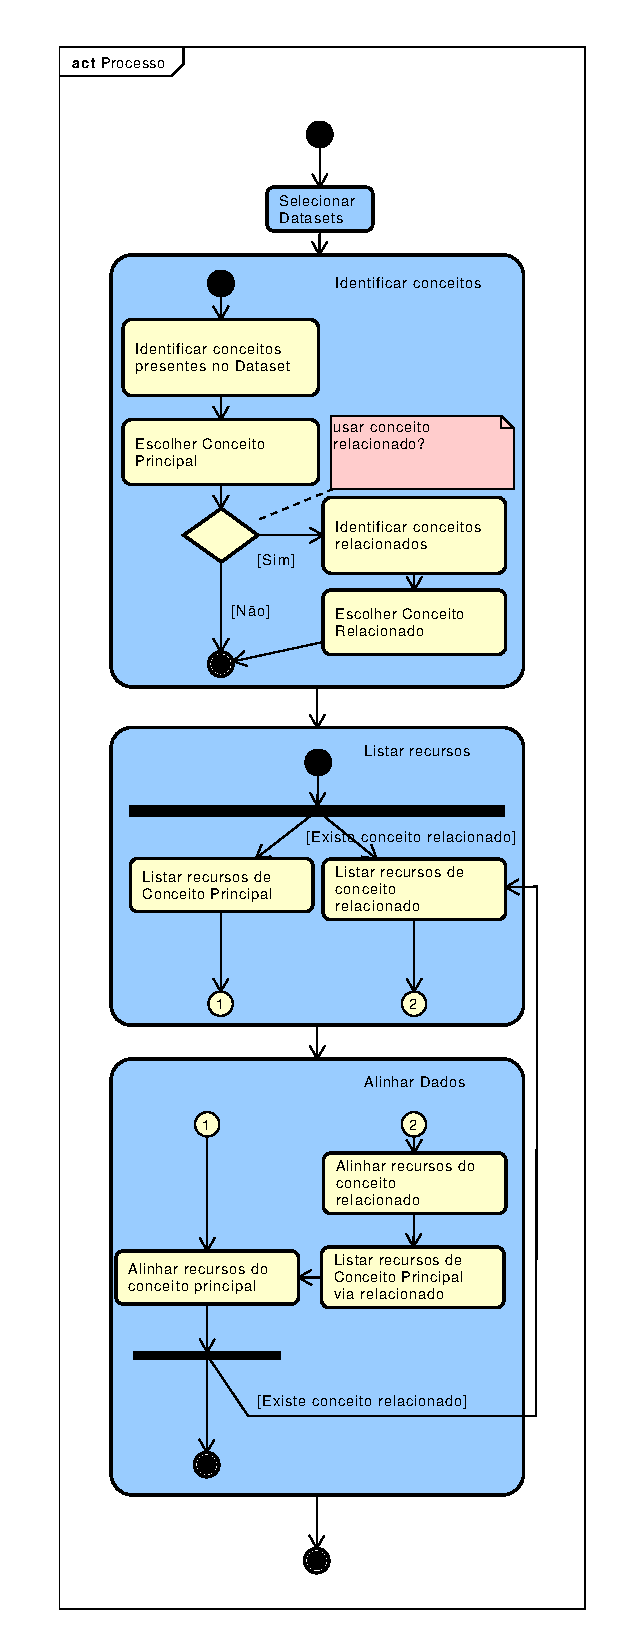
\includegraphics[width=0.55\textwidth]{./imagens/processo.pdf}
    \caption{Processo de alinhamento de dados conectados}
	\label{fig:processo}
\end{figure}

\subsection{I - Selecionar Conjunto de Dados}
A etapa de selecionar \textit{datasets} visa determinar quais conjuntos de dados serão alinhados. A seleção de um \textit{dataset} está sujeita a alguns critérios, tais como: estar estruturado em triplas e utilizar conceitos modelados em ontologias/vocabulários. 

Tais critérios foram definidos de acordo com o escopo do processo, ou seja, dados conectados. Nesta área, há ferramentas e processos disponíveis para a publicação de dados conectados na Web, que apesar de estar relacionado ao trabalho proposto não pertence ao escopo do mesmo. Além disso, é importante destacar que ao modelar os dados em qualquer processo de publicação de dados conectados são utilizadas ontologias/vocabulários que podem servir como base. Complementarmente, além de se adequar ao escopo, os critérios cumprem os requisitos mínimos para a execução do processo. 

\subsection{II - Identificar Conceitos}
\label{sec:prop_identificar}
Para auxiliar na escolha do conceito principal bem como os conceitos que estão relacionados, foram desenvolvidas duas consultas SPARQL. A primeira consulta explora a ontologia, principalmente as relações \textit{rdfs:domain} e \textit{rdfs:range} das propriedades de objeto (ver código \ref{lst:sparql}). A segunda explora os dados e as relações estabelecidas pelas instâncias.
Na consulta (código \ref{lst:sparql}), a linha 4 tem o papel de recuperar todos os conceitos pertencentes à ontologia ou vocabulário. Na linha 5 é aplicada uma restrição, em que os conceitos devem ser domínio ou \textit{range} de uma relação. Consequentemente, uma instância desse conceito será sujeito ou objeto de uma tripla (ver Figura \ref{fig:subgrafo}).
% * <profsean@gmail.com> 2017-01-18T23:27:16.703Z:
% 
% > linha 4
% Então o código deveria ter as linhas numeradas...
% 
% ^ <armandobs14@gmail.com> 2017-01-20T04:21:45.614Z:
%
% O número das linhas foi adicionada.
%
% ^ <armandobs14@gmail.com> 2017-01-20T04:21:46.821Z.
\begin{figure}[!h]
	\centering
	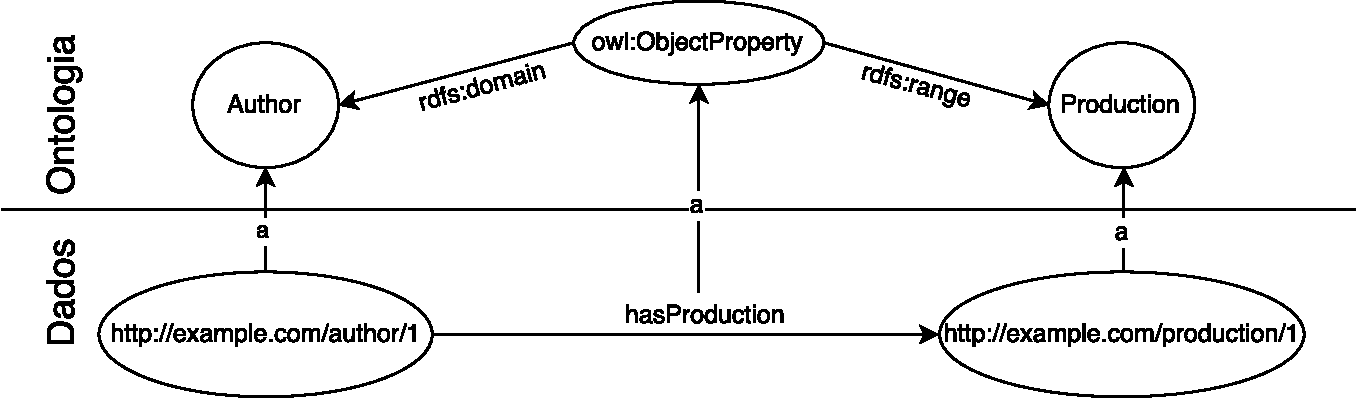
\includegraphics[width=0.9\textwidth]{./imagens/subgrafo_semantico.pdf}
	\caption{Relação entre ontologia e dados}
	\label{fig:subgrafo}
\end{figure}

\begin{lstlisting}[float,captionpos=b, caption= Consulta SPARQL para identificação de conceito, label=lst:sparql,
% * <profsean@gmail.com> 2017-01-18T23:29:21.615Z:
% 
% > lstlisting
% Não deveria estar "Código" na legenda, ao invés de "Listing"?
% 
% ^ <armandobs14@gmail.com> 2017-01-20T04:22:18.738Z:
% 
% 
% 
% ^ <armandobs14@gmail.com> 2017-01-20T04:22:20.596Z:
%
% O comando foi renomeado de listing para código.
%
% ^ <armandobs14@gmail.com> 2017-01-20T04:22:32.874Z.
basicstyle=\ttfamily,frame=single]
PREFIX rdf: <http://www.w3.org/1999/02/22-rdf-syntax-ns#>
PREFIX rdfs: <http://www.w3.org/2000/01/rdf-schema#>
select distinct ?Concept count(*) as ?count where {
[] 	a ?Concept.
?Concept 	(^rdfs:domain|^rdfs:range) ?o.
}
group 	by ?Concept	
order 	by desc(?count)
\end{lstlisting}

A consulta apresentada no Código \ref{lst:sparql2} é composta de duas partes, visto que o conceito pode modelar instâncias que são sujeito ou objeto de uma relação. Na primeira parte, o conceito selecionado representa o sujeito da tripla. Através das relações das instâncias é possível recuperar os conceitos que modelam as instâncias  relacionadas (objetos). Na segunda parte ocorre o inverso, o conceito representa o objeto da tripla e os conceitos que representam os sujeitos são recuperados.

\begin{lstlisting}[captionpos=b, caption=Query SPARQL para recuperação de conceitos relacionados, label=lst:sparql2,
   basicstyle=\ttfamily,frame=single]
PREFIX rdf: <http://www.w3.org/1999/02/22-rdf-syntax-ns#>
PREFIX rdfs: <http://www.w3.org/2000/01/rdf-schema#>


select distinct ?type where {
	values ?Concept{<URI do conceito escolhido>}
	{
		?instance rdf:type ?Concept; ?p ?o.
		?p rdf:type owl:ObjectProperty.
		?o rdf:type ?type.
	}
	union
	{
		?s ?p ?o.
		?p rdf:type owl:ObjectProperty.
		?o rdf:type ?Concept.
		?s rdf:type ?type.
	}
}

\end{lstlisting}

Como resultado do Código \ref{lst:sparql2} é provida uma lista contendo os conceitos relacionados ao conceito (principal) escolhido. Neste momento, o usuário deve escolher, quais conceitos relacionados ele deseja utilizar para melhorar o alinhamento do conceito escolhido. A escolha dos conceitos, assim como a quantidade de conceitos relacionados pode ser realizada de forma arbitrária. Essa decisão influenciará tanto no tempo que o processo levará para concluir, quanto na quantidade de recursos alinhados ao final do processo, pois para cada conceito relacionado haverá uma nova execução das etapas (iii) e (iv). Esse \textit{loop} é necessário, pois alguns alinhamentos serão possíveis apenas através da relação entre esses conceitos.

\subsection{III - Listar Recursos}
A etapa de listar recursos pode ser entendida como a recuperação dos recursos que pertencem aos conceitos. É importante destacar que a listagem/recuperação de recursos da base de conhecimento pode ser executada mais de uma vez durante o processo, gerando um conjunto de recursos para cada conceito escolhido. Além disso, essa etapa é responsável pela geração de pares candidatos, onde os recursos do \textit{Dataset} $D_{1}$ são comparados com os recursos do \textit{Dataset} $D_{2}$.


\subsection{IV - Alinhar Dados}
A etapa de alinhamento de dados está dividida em duas atividades sendo elas: (i) alinhamento simples e (ii) alinhamento em cascata, que serão detalhados nas subseções a seguir.

\subsubsection{Alinhamento simples}
\label{im_simples}
Para alinhar os recursos é necessário executar alguns procedimentos, sendo eles o tratamento dos dados, comparação entre recursos e análise da similaridade. O primeiro procedimento, tratamento, se refere a transformações nas propriedades dos recursos. Essas transformações são necessárias para auxiliar os algoritmos de similaridade a analisarem melhor a semelhança entre os recursos. No procedimento de comparação, cada uma da propriedades é analisada. Caso uma propriedade não pertença a um dos recursos, ela é dispensada da comparação. A Figura  \ref{fig:resources} apresenta a comparação entre as propriedades de cada recurso.

\begin{figure}[!h]
	\centering
	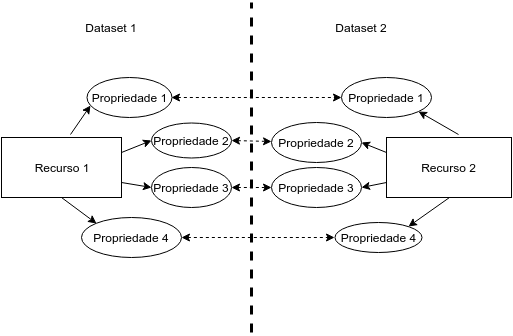
\includegraphics[width=0.6\textwidth]{./imagens/resources.png}
    \caption{Comparação entre recursos}
	\label{fig:resources}
\end{figure}

Para definir a similaridade entre as instâncias foram usadas duas equações. A Equação \ref{eq:properties_definition} define o conjunto de propriedades que será considerado durante a comparação entre os recursos, que será obtido a partir da diferença entre  o maior conjunto de propriedades e o conjunto de propriedades que deve ser desconsiderado. Logo:

\begin{equation}
P_f =M a x  ( P_{r1} ,P_{r2} ) - P_d
\label{eq:properties_definition}
\end{equation}

Onde:
\begin{itemize}
	\item $P_{r1}$ – Conjunto de propriedades do recurso 1;
	\item $P_{r2}$ – Conjunto de propriedades do recurso 2;
	\item $P_d$ –  Conjunto de propriedades que devem ser desconsideradas;
	\item $M a x  ( P_{r1} ,P_{r2} )$ – Retorna o conjunto com maior número de propriedades;
\end{itemize}

A Equação \ref{eq:similaridade} trata da função de similaridade entre recursos, essa equação pode ser entendida como a média das similaridades entre dois recursos. Tal abordagem foi escolhida com o objetivo de não privilegiar nenhuma das similaridades parciais. Contudo, é possível que existam outras funções mais adequadas para calcular a similaridade entre recursos.
% * <profsean@gmail.com> 2017-01-18T23:53:58.395Z:
% 
% > média
% Por que média? Talvez outras medidas tenham resultado melhor...
% 
% ^ <armandobs14@gmail.com> 2017-01-20T04:39:25.946Z:
%
% Foi comentado que a média foi utilizada com o objetivo de não privilegiar nenhuma das similaridades parciais. Também foi reconhecido que podem existir funções mais adequadas para calcular a similaridade entre recursos.
%
% ^ <armandobs14@gmail.com> 2017-01-20T04:40:23.851Z.

\begin{equation}
SR  = \frac{1}{|P_f|} { \sum_{i = 1}^{P_f} {S(V(R_1,P_f[i]);V(R_2,P_f[i]))}}
\label{eq:similaridade}
\end{equation}

Onde:

\begin{itemize}
	\item S – Função de similaridade;
% * <profsean@gmail.com> 2017-01-18T23:54:38.751Z:
% 
% > similaridade léxica
% Por que somente similaridade léxica? Poderia ser qualquer tipo, inclusive um conjunto de similaridades... Entendo que na implementação vc tratou somente a léxica, mas em termos de proposta não há essa limitação...
% 
% ^ <armandobs14@gmail.com> 2017-01-20T04:42:23.315Z:
%
% Concordo. acredito que a restrição de similaridade léxica esteja apresentada apenas neste ponto.
%
% ^ <armandobs14@gmail.com> 2017-01-20T04:42:24.935Z.
	\item V(R,P) – Valor da propriedade P em um recurso R;
	\item $R_1$ – Recurso 1;
	\item $R_2$ – Recurso 2;
\end{itemize}

O valor gerado pelo componente de similaridade é enviado para o componente de alinhamento.

\subsubsection{Alinhamento em cascata}
\label{sub:cascata}
O alinhamento em cascata recebe esse nome devido ao encadeamento entre as atividades necessárias: (i) Recuperar instâncias que pertencem ao conceito relacionado; (ii) Alinhar instâncias que pertencem ao conceito relacionado; (iii) Recuperar instâncias que pertencem ao conceito principal; e (iv) Alinhar instâncias que pertencem ao conceito principal. O nome também foi utilizado com a intenção de fazer referência ao modelo de desenvolvimento em cascata \cite{royce1970managing}, que é o primeiro modelo de desenvolvimento de software. Segundo \citeonline{sommerville2011software}, trata-se de um modelo dirigido por planos, cujas etapas são planejadas antes da execução. 

O modelo de desenvolvimento em cascata e a abordagem de alinhamento em cascata compartilham algumas semelhanças. Dentre as semelhanças compartilhadas, temos o modo como as atividades são executadas, que é sequencial. Além disso, cada atividade só pode ser iniciada quando a atividade anterior for concluída. Outra característica compartilhada entre eles é o fato de todo o projeto ser planejado antes da execução. 

Diferentemente de um projeto que utiliza o modelo em cascata, onde todo o projeto deve estar concluído na etapa final, tem-se que o processo de correspondência entre instâncias só será considerado concluído quando todos os conceitos relacionados forem utilizados no processo de correspondência. Vale ressaltar que uma “cascata” é gerada para cada conceito relacionado selecionado. 

A Figura \ref{cp_cascata} apresenta o relacionamento entre os conceitos e a cascata.

\begin{figure}[!h]
	\centering
	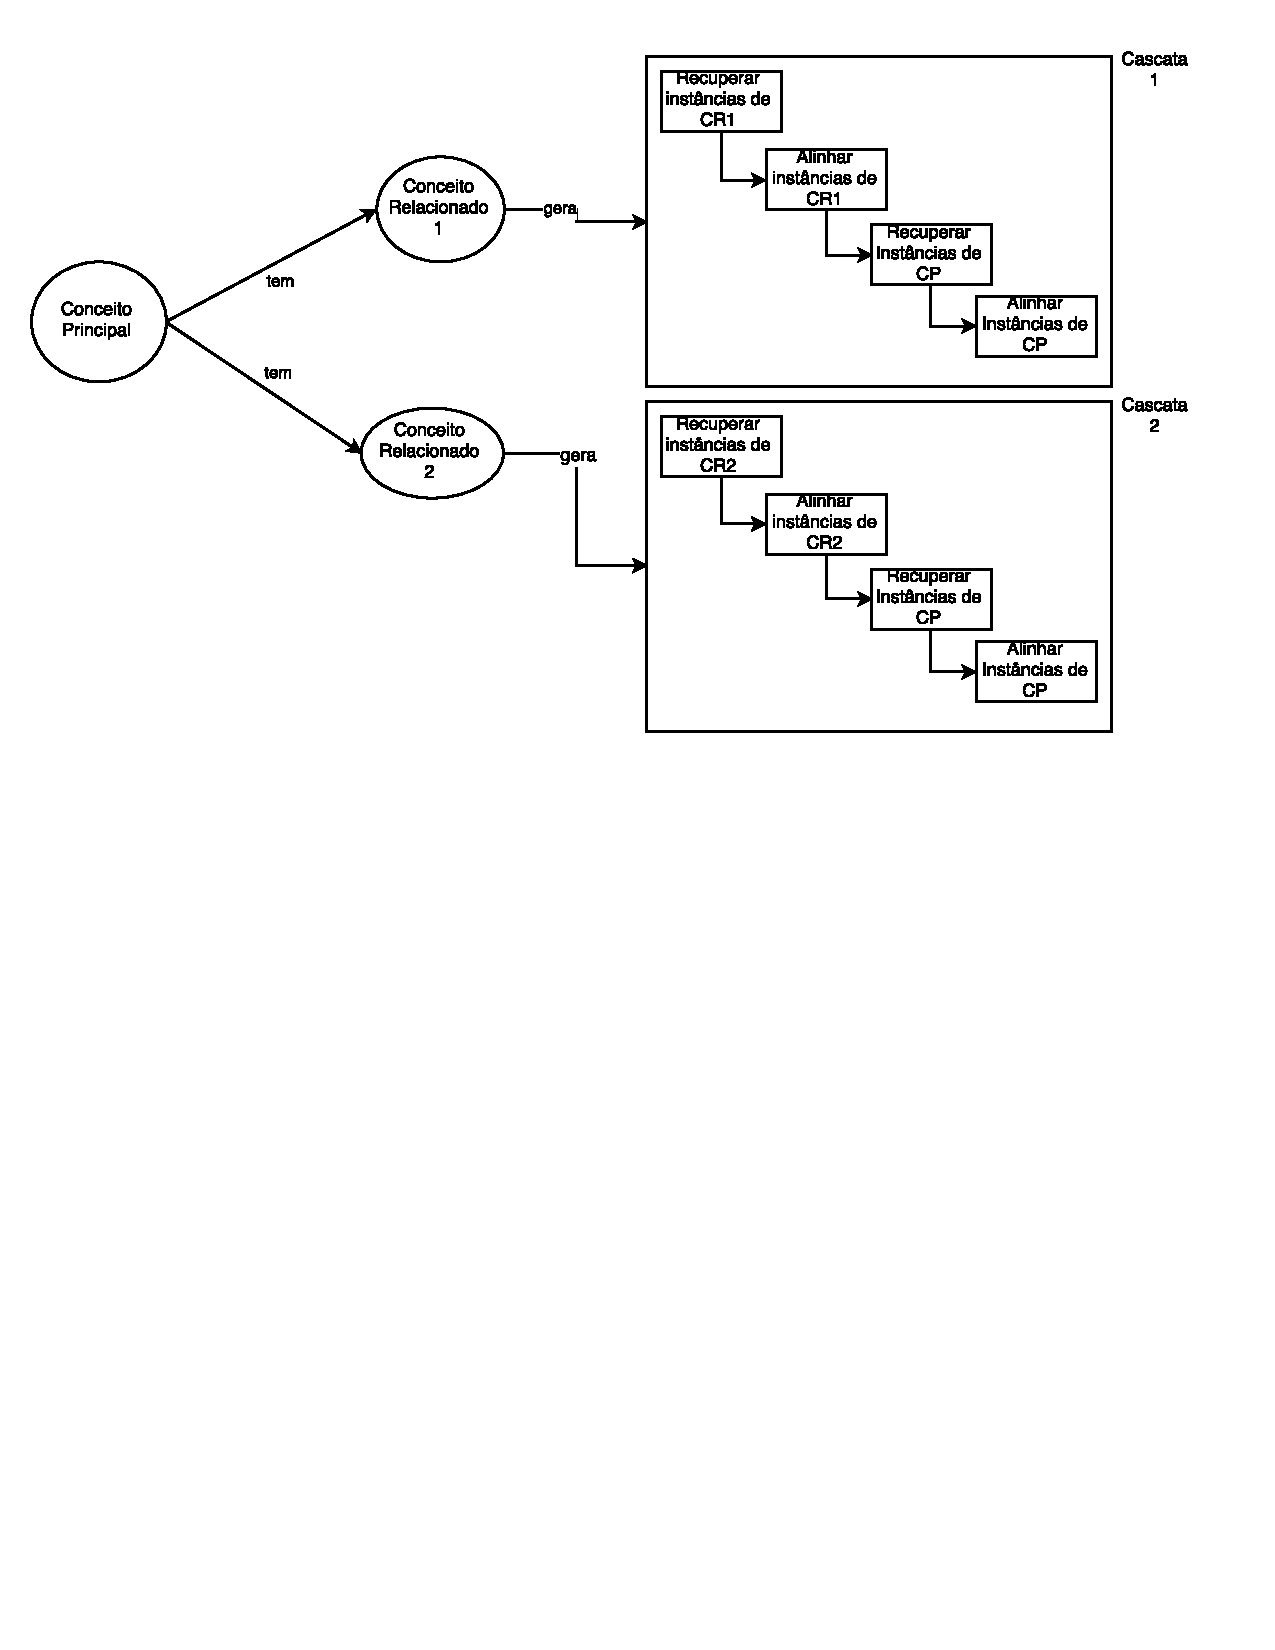
\includegraphics[width=1\textwidth]{./imagens/CM_cascata.pdf}
	\caption{Relacionamento entre conceito relacionado e cascata}
	\label{cp_cascata}
\end{figure}

Imaginemos que algum órgão deseja encontrar quais autores estão presentes em dois \textit{datasets} simultaneamente. Para isso, desejam utilizar os artigos presentes em ambas as bases. Dessa forma, temos que o conceito principal e conceito relacionado são \textbf{\textit{Author}} e \textbf{\textit{Publication}}, respectivamente.

%\subsubsection{Recuperar Instâncias do Conceito Relacionado}
\paragraph{Recuperar Instâncias do Conceito Relacionado}
\label{recuperao_relacionado}
Nesta atividade recuperam-se as instâncias que pertencem a um conceito relacionado. Para isso, consultas são realizadas nos \textit{datasets} selecionados na primeira etapa do processo.  Os resultados das buscas são agrupados em listas, uma para cada \textit{dataset}. Cada elemento da lista é um grafo que é composto pela instância e seus relacionamentos. Por fim, as listas são enviadas para a próxima atividade da cascata, como pode ser visto na Figura \ref{cp_cascata}.

Tomando como referência o exemplo citado, temos que as listas serão compostas por instâncias de \textbf{\textit{Publication}} e seus relacionamentos.

%\subsubsection{Alinhar Instâncias do Conceito Relacionado}
\paragraph{Alinhar Instâncias do Conceito Relacionado}
\label{lista_rel}

As instâncias recuperadas na atividade \ref{recuperao_relacionado} são submetidas para o alinhamento. Através do cálculo de similaridade realizado entre essas instâncias. O resultado desse cálculo é comparado com um limiar de aceitação, havendo duas possibilidades. Em caso positivo, ou seja, a similaridade está no limiar de aceitação. Consequentemente, as instâncias são entendidas como correspondentes e o alinhamento é persistido. Caso contrário, o par candidato é descartado.

%\subsubsection{Recuperar Recursos do conceito principal}
\paragraph{Recuperar Recursos do conceito principal}
\label{recuperao_principal}

Similarmente ao que ocorre na subseção \ref{recuperao_relacionado}, a recuperação  das instâncias que pertencem ao conceito principal (\textbf{\textit{Author}}) também é realizada através de consultas nos \textit{datasets} selecionados. Porém, neste caso, as instâncias recuperadas devem estar relacionadas às instâncias da correspondência persistida anteriormente. Dessa forma, os autores que estão relacionados à publicação são recuperados e agrupados de acordo com o \textit{dataset}. A Figura \ref{fig:relacionados} apresenta a relação entre as instâncias que pertencem ao conceito principal e as correspondências.

\begin{figure}[!h]
	\centering
	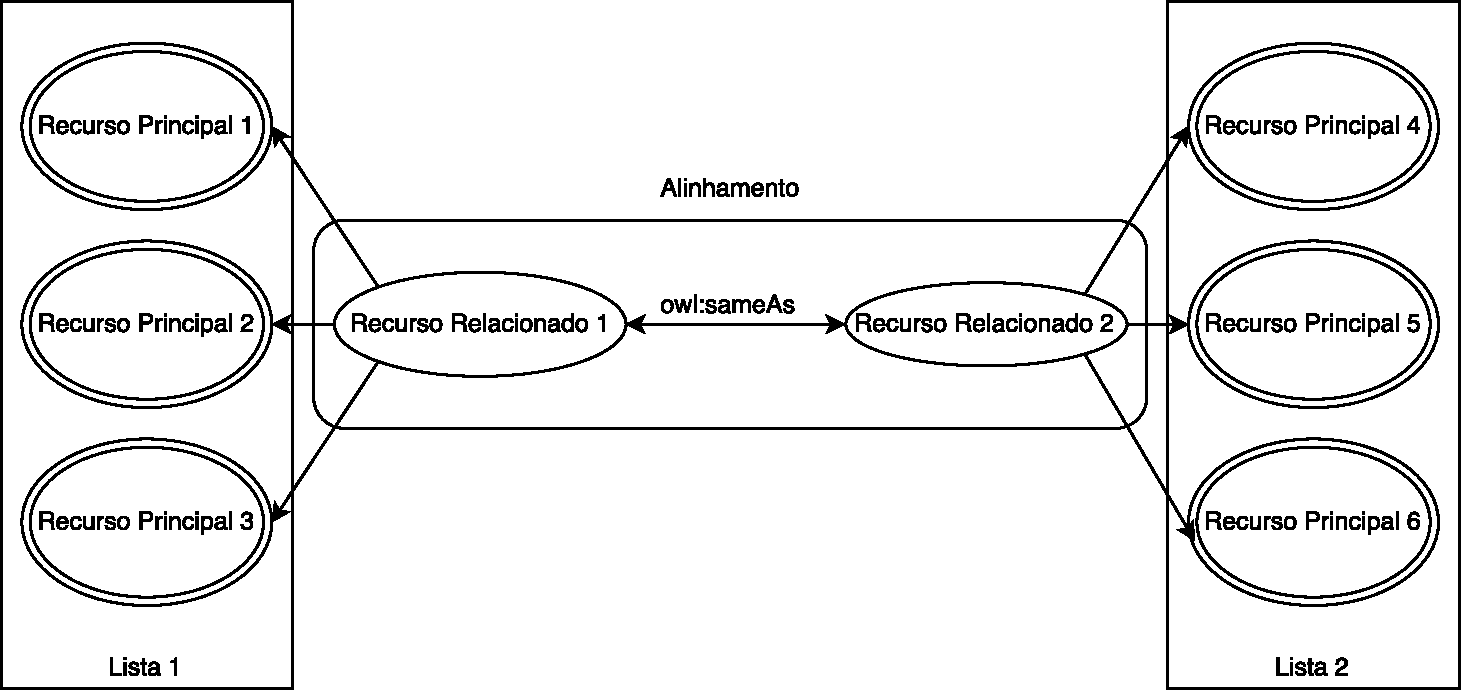
\includegraphics[width=0.9\textwidth]{./imagens/relacionados.pdf}
	\caption{Relacionamento entre instâncias e correspondência}
	\label{fig:relacionados}
\end{figure}

%\subsubsection{Alinhar Recursos Recuperados}
\paragraph{Alinhar Recursos Recuperados}

Através da restrição aplicada na atividade \ref{recuperao_principal}, tem-se que as instâncias recuperadas estão relacionadas à mesma entidade do mundo real. Consequentemente, existe ao menos uma correspondência entre as instâncias recuperadas. Assim, a correspondência entre os autores é persistida. 
% * <profsean@gmail.com> 2017-01-19T00:14:52.107Z:
% 
% > persistida
% Senti falta de uma seção de encerramento do capítulo...
% 
% ^ <armandobs14@gmail.com> 2017-01-19T20:07:37.053Z:
%
% Foi adicionada uma seção de considerações finais.
%
% ^ <armandobs14@gmail.com> 2017-01-20T04:43:12.263Z.
\section{Considerações Finais}
Este capítulo apresentou um processo para o alinhamento de dados. Este processo foi projetado para permitir que soluções sejam capazes de estabelecer a correspondência entre instâncias dispensando a utilização de computação específica, em outras palavras, permitindo que as aplicações sejam livres de contexto. O processo foi dividido em quatro etapas (Selecionar \textit{datasets}, Identificar conceitos, Recuperar instâncias e Alinhar dados).  A etapa de alinhamento, por sua vez é composta de duas atividades (Alinhamento Simples e Alinhamento em Cascata).

A atividade de alinhamento em cascata define um subprocesso composto por quatro atividades (Recuperar instâncias de conceito relacionado, Alinhar instâncias de conceito relacionado, Recuperar instâncias de conceito principal e Alinhar instâncias do conceito principal). De modo a apoiar a realização das subatividades, nós apresentamos uma breve descrição para cada atividade.

No próximo capítulo será apresentada uma arquitetura  que implementa o processo proposto.

